\documentclass[a4paper,12pt]{report}
\usepackage[utf8]{inputenc}
\usepackage[francais]{babel}
\usepackage{fancyhdr}
\usepackage{graphicx}
\usepackage{tikz}
\usetikzlibrary{calc}
\usepackage{listings}
\usepackage{xcolor}
\definecolor{grey}{rgb}{0.9,0.9,0.9}
\usepackage{titlesec}
\usepackage{verbatim}
\usepackage{listings}
\usepackage{textcomp}
\usepackage{hyperref}
\usepackage{longtable}
\usepackage{colortbl}
\usepackage{amssymb}

\definecolor{javakeyword}{rgb}{0,0,0.5}
\definecolor{javastring}{rgb}{0,0.5,0}
\definecolor{javacomment}{rgb}{0.5,0.5,0.5}
\lstdefinestyle{Scilab}{
   language=Scilab, basicstyle=\footnotesize,       % the size of the fonts that are used for the code
  numbers=left,                   % where to put the line-numbers
  numberstyle=\tiny\color{gray},  % the style that is used for the line-numbers
  stepnumber=1,                   % the step between two line-numbers. If it's 1, each line
                                  % will be numbered
  numbersep=5pt,                  % how far the line-numbers are from the code
  backgroundcolor=\color{white},  % choose the background color. You must add \usepackage{color}
  showspaces=false,               % show spaces adding particular underscores
  showstringspaces=false,         % underline spaces within strings
  showtabs=false,                 % show tabs within strings adding particular underscores
  frame=single,                   % adds a frame around the code
  rulecolor=\color{black},        % if not set, the frame-color may be changed on line-breaks within not-black text (e.g. commens (green here))
  tabsize=2,                      % sets default tabsize to 2 spaces
  captionpos=b,                   % sets the caption-position to bottom
  breaklines=true,                % sets automatic line breaking
  breakatwhitespace=false,        % sets if automatic breaks should only happen at whitespace
  title=\lstname,                 % show the filename of files included with \lstinputlisting;
   stringstyle=\color{javastring},
   keywordstyle=\color{javakeyword}\ttfamily\textbf,
   commentstyle=\color{javacomment}\ttfamily\textit
 }
\frenchbsetup{StandardLists=true}
\newcommand{\marge}{18mm}
\usepackage[left=\marge,right=\marge,top=\marge,bottom=\marge]{geometry}
\pagestyle{fancy}
\setlength{\headheight}{15pt}
\renewcommand{\headrulewidth}{1pt}
\linespread{1}
\setlength{\columnseprule}{0.2pt}
\title{TP1 VISA : éléments de géométrie projective et calibration de caméra}
\author{NAIT ABDELAZIZ Yanis}


\begin{document}
\maketitle
\section*{Introduction}
Dans ce TP, nous allons opérer à la calibration d'une caméra en utilisant la méthode de zhang. La calibration d'une caméra consiste en effet à determiner les paramètres intrinsèques et extrinsèques de celle-ci en effectuant quelques calculs matriciels sur l'image de mire ci-dessous.
\begin{figure}[!ht]
\center
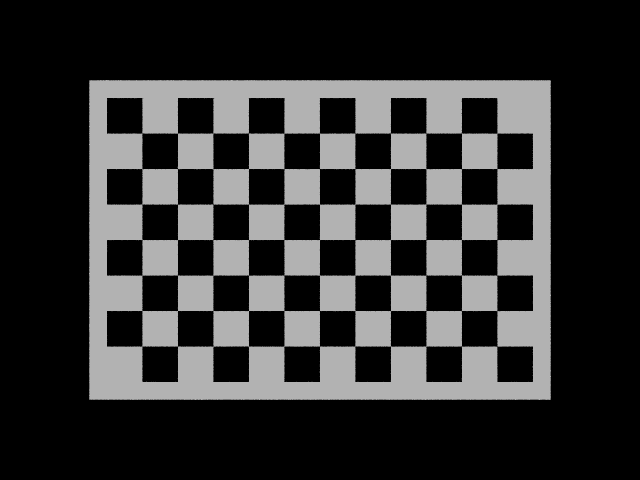
\includegraphics[scale=0.3]{./image/mire.png}
\end{figure}
\section*{Estimation des paramètres intrinsèques}
Dans un premier temps, afin d'estimer les matrice intrinsèque de la caméra nous allons tout d'abord calculer une matrice d'homographie qui est une fonction permettant de projeter des points d'un repère dans un autre repère. Cette matrice va ainsi nous permettre de poser un système d'equations de contraintes. Ainsi en résolvant ce système d'équations nous allons pouvoir déterminer les différentes valeurs contenues dans la matrice intrinsèque de la caméra. Enfin la matrice extrinsèque pourra être calculée facilement.
\subsection*{Q1}
Après analyse du code fourni, on voit que toutes les étapes décrites ci-dessus ont été implémentées dans le même ordre:

\begin{lstlisting}[style=Scilab]
/*****Matrice d'homographie*****/
H = zeros(3, 3, ni);
m = zeros(3, np, ni);
for i = 1:ni
  // Lire les points de l'image
  m(1:2,:,i) = read('points-'+string(i)+'.txt', -1, 2)';
  m(3,:,i) = ones(1, np);
  // Estimer l'homographie entre la mire et l' image
  H(:,:,i) = ZhangHomography(M(sansZ,:), m(:,:,i));
  // Ajouter deux lignes de contraintes dans V
  V = [V; ZhangConstraints(H(:,:,i))];
end

/*****Matrice intrinseque******/
A = IntrinsicMatrix(b);

/*****Matrice extrinseque*****/
E = zeros(3, 4, ni);
for i = 1:ni
  E(:,:,i) = ExtrinsicMatrix(iA, H(:,:,i));
end 
\end{lstlisting}

\subsection*{Q2}

Le code ci-dessous permet d'établir le système d'équations de contrainte comme énoncé dans la méthode de Zhang. Ces équations sont stockés dans un vecteur ligne afin de faciliter les calculs par la suite: 
\begin{lstlisting}[style=Scilab]
function v = ZhangConstraintTerm(H, i, j)
  a = H(1,i)*H(1,j);
  b = H(1,i)*H(2,j)+H(2,i)*H(1,j);
  c = H(2,i)*H(2,j);
  d = H(3,i)*H(1,j)+H(1,i)*H(3,j);
  e = H(3,i)*H(2,j)+H(2,i)*H(3,j);
  f = H(3,i)*H(3,j);
  v = [a,b,c,d,e,f];
endfunction
\end{lstlisting}

\subsection*{Q3}
Le code ci-dessous va permettre de calculer à partir du vecteur b calculé précedemment la matrice intrinsèque de la manière suivante:
\begin{lstlisting}[style=Scilab]
function A = IntrinsicMatrix(b)
  _v0 = (b(2)*b(4)-b(1)*b(5))/(b(1)*b(3)-b(2)*b(2));
  _lambda = b(6)-(b(4)*b(4)+_v0*(b(2)*b(4)-b(1)*b(5)))/b(1);
  _alpha = sqrt(_lambda/b(1));
  _beta = sqrt((_lambda*b(1))/(b(1)*b(3)-b(2)*b(2)));
  _gamma = -(b(2)*_alpha*_alpha*_beta/_lambda);
  _u0 = _gamma*_v0/_beta - b(4)*_alpha*_alpha/_lambda; 
  
  A =[_alpha,_gamma,_u0;
      0,_beta, _v0;
      0,0,1];
endfunction
\end{lstlisting}
\subsection*{Q4}
Ci-dessous, les matrices intrinsèques A et B calculées respectivement par la méthode de Zhang et la méthode de Povray:\\
\begin{center}
\[
	A=\left (
	\begin{array}{ccc}
		3498.2767 & - 3.13105  &  336.76583 \\  
        0.        &  3503.8946 & 220.1142 \\   
        0.        &   0.     &      1.       \\
	\end{array}
	\right )	
\]
\[
	B=\left (
	\begin{array}{ccc}
		3546.099291 & 0.000000    & 320.000000    \\
		0.000000    & 3546.099291 & 240.000000   \\
		0.000000    & 0.000000    & 1.000000    \\
	\end{array}
	\right )
\]
\end{center}
On remarque que les valeurs des éléments des ces deux matrices sont très proches. On peut donc dire que la méthode de Zhang implémentée est satisfaisante pour estimer la matrice intrinsèque de la caméra.

\section*{Estimation des paramètres extrinsèques}
Dans cette, nous allons enfin pouvoir calculer la matrice extrinsèque de la caméra grâce à l'inverse de la matrice intrinsèque iA calculée précedemment et la matrice d'homographie H. 
\subsection*{Q1}
Le code ci-dessous décrit cette dernière étape de calibration:
\begin{lstlisting}[style=Scilab]
function E = ExtrinsicMatrix(iA, H)
  lambda = 1/abs(iA*H(:,1));
  lambda = lambda(1);
  r1 = lambda * iA * H(:,1);
  r2 = lambda * iA * H(:,2);
  r3 = CrossProduct(r1,r2);
  t = lambda * iA * H(:,3);
  E  = [r1,r2,r3,t]; 
endfunction
\end{lstlisting}
\subsection*{Q2}
Ci-dessous, on voit les matrices extrinsèques A et B correspondant respectivement à celle que nous avons calculée avec la méthode de Zhang et à celle qui nous a été fournie:\\
\begin{center}
\[
	A=\left (
	\begin{array}{cccc}
		1.           & 0.0009052  & - 0.0006686 &  - 48.811577 \\
		0.0000377    & 0.9982951  &  0.0015769  &  54.73332   \\
		0.0006696  & - 0.0015763  &  0.9982950  &  9854.3628  \\
	\end{array}
	\right )	
\]
\[
	B=\left (
	\begin{array}{cccc}
		0.0 & 0.0 & 0.0 & 0.0    \\
		0.0 & 0.0 & 0.0 & 0.0  \\
		0.0 & 0.0 & 0.0 & 10000  \\
	\end{array}
	\right )
\]
\end{center}
Par comparaison, on peut voir que les deux résultats sont encore sensiblement proches. Ce qui nous permet de confirmer de l'efficacité de la méthode de calibration exposée par Zhang.

\section*{Conclusion}
On peut conclure sur le fait que la méthode de calibration proposée par Zhang fournit des résultats satisfaisants par rapport aux résultats théoriques. L'introduction de caractéristiques réelles dans la méthode de Zhang permettrait de tendre vers de meilleurs résultats.
\end{document}